\chapter{Utvalgte situasjoner i prosjektperioden}

\section{Case 1 - En krangel mellom Håkon og Ali}

\subsection{Situasjon}


Klokka nærmer seg 15.30 og alle gruppemedlemmer kjenner at det har vært en lang og tung dag. Vi har jobbet iherdig gjennom dagen. Første halvdel gikk til prosjektoppgaven mens etter lunsj ble satt av tid til å diskutere vårt siste case. Det ble diskutert i nærmere èn og en halv time rundt temaet Alis forsentkomminger. Her kom det fram at gruppemedlemmene hadde forskjellige holdninger til å møte til avtalt tid. Det var en meget konstruktiv diskusjon med mange forskjellige synsvinkler og meninger. Her tenkte vi at vi virkelig hadde noe å skrive om, som kunne reflektere forskjellene mellom gruppemedlemmene. Vi var fornøyde og ble enige om å ta en kort pause, for så å gjenoppta diskusjonen. Jonas går en tur på toalettet, Anders går for å hente seg litt vann og Ali benytter pausen på å fullføre noe på datamaskinen. I det pausen er over og Jonas og Anders er kommet tilbake, blir Ali oppringt på telefonen. Han ser på telefonen og lurer på hvem det er som ringer. Han svarer ikke på telefonen og Håkon initierer gjenopptagelsen av diskusjonen vi skulle ha etter pausen. I det Håkon begynner å prate og ser seg rundt bordet for å fange øyekontakt med gruppemedlemmene, ser han at Ali sitter og tekster på telefonen.\\

\textit{"Ali, nå må du legge ned den telefonen og følge med! Samma om det er for en sommerjobb eller et annet fag, vi har blitt enige om at når vi diskuterer sammen så skal alle følge med."}{--Håkon}\\

Det blir med en gang stille i gruppen og Ali sine øyne spretter opp. Det går et sekund eller to før Ali helt får med seg hva som har skjedd. Jonas, Anders og Lars sitter med hodet lett presset bak, overrasket over situasjonen. Håkon virker passe irritert, og ønsker at gruppa skal følge det vi har sagt tidligere om at alle skal følge med når gruppa i felleskap diskuterer.\\

\textit{"Håkon, nå må du roe deg ned. Nå må du seriøst roe deg ned."}{--Ali}\\

Jonas bemerker seg at situasjonen begynner å gå opp for Ali, og synes han ser en irritasjon bygge seg opp i Ali etterhvert som han får tenkt litt på hva som har skjedd. Anders er redd for at situasjonen skal eskalere, og at det framtidige samarbeidet i gruppen står i fare. Anders legger spesielt merke til at stemmebruken og temperaturen er litt høyere enn hva han er komfortabel med.\\

\textit{"Når vi har blitt enige om at alle skal følge med når noen snakker, så syns jeg vi skal følge det, uansett hva det er"}{--Håkon}\\

\textit{"Noen prøvde å ringe meg, og jeg skulle bare svare og si at jeg var opptatt, og at jeg skulle ringe tilb... jeg behøver ikke å forklare meg for deg på denne måten for faen"}{--Ali}\\

Ali kaster oppgitt fra seg pennen han holder i hånden og ser ned i bordet og rundt i rommet med frustrasjon. Håkon prøver å forklare hvorfor han sa det han sa, og stod fortsatt for det han mente. Ali var fortsatt meget provosert og hintet til at dersom Håkon ikke sluttet å snakke, så ville han få en mobiltelefon servert i skallen. Lars, Anders og Jonas tenkte at det nå var lurt å ta en liten pause til for å roe seg ned. Deretter kunne vi så skrive ned situasjonen for å ta den opp og diskutere hva som hadde skjedd når ting kjølte seg litt ned.

\newpage

\subsection{Refleksjoner}

Sett tilbake på denne hendelsen, er det mange ting man kan spørre seg om hva som kunne blitt gjort annerledes eller bedre for å unngå en slik direkte konfrontasjon. Skjedde dette spontant, eller var det en reaksjon på noe som hadde bygget seg opp over lengre tid? Uken etter denne hendelsen tok vi opp temaet på nytt og snakket gjennom det i en mer nøytral og reflekterende forstand. Denne uka var Lars borte, men resten av gruppa satt en god halvtime og diskuterte hvorfor de trodde hendelsen utspilte seg som den gjorde. Vi startet med å ta runden rundt bordet og la hver person forklare hva de syntes om situasjonen.\\

Det startet med Anders og Jonas sine gjenfortellinger av situasjonen, som var ganske like. Anders mente han opplevde at Håkon kjeftet på Ali i måten han uttalte seg på og poengterte at han selv ikke ville likt å bli snakket til å den måten. Han hadde forståelse for at Ali ble provosert og reagerte på måten han gjorde, men hadde foretrukket at temperaturen hadde vært noe lavere. Jonas mente mye av det samme, og følte seg og ganske ukomfortabel i situasjonen. Han observerte en klar misnøye fra Ali grunnet måten han ble konfrontert, men tenkte at han kanskje ikke ville reagert like sterkt selv. Dette tror han grunner i at hans egen far har hatt et ganske likt atferdsmønster gjennom oppveksten, der små irritasjonsmoment bygget seg opp til en eksplosjon. Jonas tror dermed det gjorde denne situasjonen mindre betydningsfull for ham selv.\\

Under refleksjonssamtalen kom det fram at Håkon og Ali hadde tydelig forskjellige forventninger til gruppas sosiale protokoller. Håkon hadde allerede på starten av semesteret fått kommunisert gjennom bli-kjent-fasen at han framstod som en ganske direkte type. Han betegnet seg selv som målfokusert, og at det var den viktigste verdien. Han vet med seg selv at når tålmodigheten strekkes kan denne direkteheten komme fram, da gjerne ufiltrert.
Ali hadde ikke hatt noen innvendinger tidligere angående viktigheten av å være punktlig, men skjønte at det var viktig for å ha god stemning i gruppa og kunne gjøre et godt arbeid. Når vi ser tilbake på samarbeidsindikatorene som vi tok gjennom semesteret, ser vi at vi ikke scoret så høyt på kategorien "ærlig og direkte". Mye av dette var nok nettopp fordi vi ikke ønsket å være for direkte. Dette mente vi var viktig for å holde god stemning innad i gruppa. Man kan kanskje si at Håkons utbrudd var en avstikker fra hva som var vanlig i gruppa, og da ikke minst utenfor forventningene til gruppa. Noe av det Lars, Anders og Jonas reagerte på, var at det tilsynelatende kom ut av det blå.\\

\begin{figure}[H] 
    \centering
    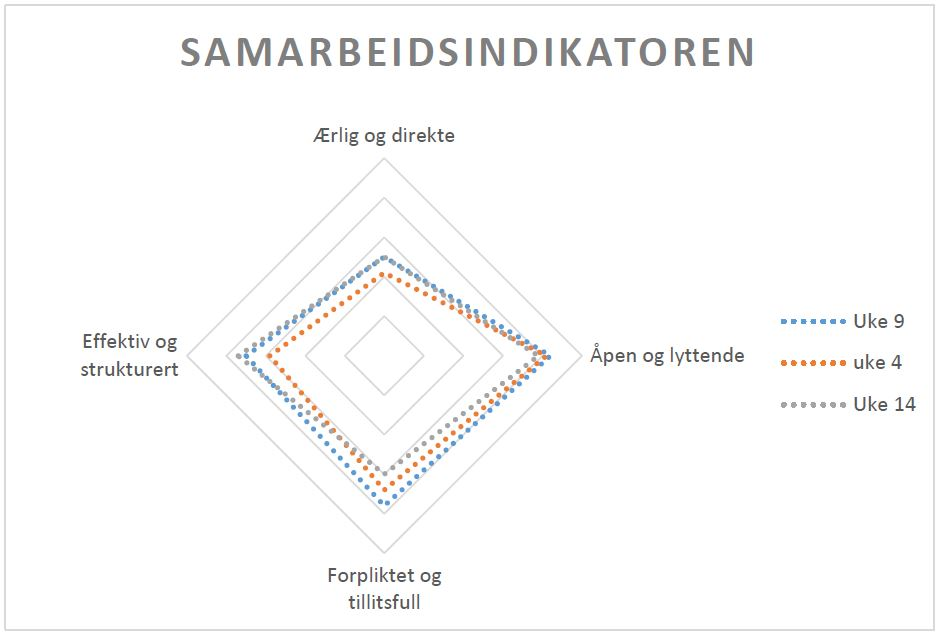
\includegraphics[scale=0.6]{images/samind2.JPG}
    \caption{Gruppas diagram fra samarbeidsindikatoren.}
    \label{fig:my_label}
\end{figure} 

\newpage

 Ut ifra hva som ble sagt i situasjonen var Håkon veldig ærlig og direkte, mer enn hva "normalen" for gruppa var. Dette kom kanskje som en respons på at Ali også hadde vært utenfor "normalen" med tanke på struktur da han gjentatte ganger hadde kommet for sent og ikke fulgt avtalen om å ikke holde på med mobilen når andre snakker. Dermed oppsto det en mismatch i samarbeidsindikatoren som kan ha ført til at situasjonen oppsto i utgangspunktet. \\

 Underveis i samtalen beklaget Håkon seg for måten han hadde ordlagt seg på og hadde forståelse for og syntes det var leit at det ble oppfattet som kjefting. I situasjonen var ikke Håkon så opptatt av hvordan budskapet skulle mottas så lenge det ble mottakeren hadde forstått budskapet og tatt dette til følge. Håkon, målbevisst som han er, var mer opptatt av å løse det underliggende "problemet", enn å tenke på hvordan det ville bli lagt fram. Ali ble på den andre siden så opprørt av tonen til Håkon at han ikke fikk med seg innholdet av det han sa, men heller måten han sa det på. Dermed handlet det for Ali heller en om hvordan han ble snakket til som person, heller enn sakens innhold.\\
 
 I forbindelse med diskusjonen om fravær nevnte Ali at nordmenn var veldig fokusert på viktigheten av å overholde avtaler som ble gjort. Dette er en observasjon flere i gruppa følte seg enig i. Anders mener at de nordiske landene generelt er mer firkantet enn resten av Europa, og verden for den del, på å være presis og å overholde avtaler. Alis lengste forsentkomming ble begrunnet med en setning som gav assosiasjoner til utsagnet \textit{"Min tid er viktigere enn din tid"}. De andres syn på forsentkomming kan gjøre at man syntes det er respektløst å ikke komme til avtalt tid, særlig hvis det skjer over flere ganger. Dermed \textit{kan} det å komme for sent tolkes som mangel av respekt for gruppas tid i fellesskap.\\
 Ali nevnte at grunnen til at han reagerte på måten han gjorde, var at han følte en mangel på respekt slik han ble snakket til. Han mente Håkon kjeftet på han og at det viser mangel på respekt.\\
 
 Begge følte da en mangel på respekt, men på forskjellige plan. Håkon fordi han følte at Ali ikke brydde seg om viktigheten med å komme tidsnok og dermed ta av fellesskapets tid, mens Ali følte en mangel av respekt fordi han følte han ble kjeftet på. \\
 
Fra kapittelet om "Valuing Diversity" i EiT-kompendiet sies det:\\

\textit{"..Bringing diverse individuals together does not result automatically in positive outcomes..."}\\{[Johnson & Johnson, 1989]}
, se \cite{EiTkomp}.\\

Her kan det tenkes at forskjellene mellom Håkon og Ali både personlig og kulturelt kan ha gjort det lettere å skape friksjoner dem imellom. Det kommer tydelig frem at de har forskjellige forventninger til adferd og respekt. Disse forventningene har gjerne forankring i kulturen man har oppvokst i.\\
 
Hvordan har disse situasjonene gitt utslag på gruppa som helhet over hele semesteret? I figur 3.1 ser vi utviklingen av samarbeidsindikatoren over tid. Det er ikke store endringer å spore men det punktet med størst variasjon er variabelen "Forpliktet og tillitsfull". Særlig ser vi at denne indikatoren har fått seg en knekk ved den siste målingen og gått ned noen poeng. Dette tror vi skyldes at tilliten innad i gruppa sank etter at denne situasjonen dukket opp, noe som er uheldig.


\newpage

\subsection{Aksjoner}


Denne hendelsen skjedde på en av landsbyens siste dager. Det ble dermed ikke diskutert så mye om hvordan vi kunne jobbe for å unngå en slik situasjon videre, siden det ikke var så mye tid igjen. Det ble generelt lagt vekt på at man skal respektere at hverandre er - og fungerer - forskjellig. At det kan være viktig å være litt varsom på- eller tenke seg om en ekstra gang før man ytrer noe.\\\\

Dersom vi skulle videreført vårt prosjektarbeid, hadde vi derimot et forslag til hvordan å takle slike situasjoner bedre i framtiden. En av øvelsene vi ble presentert for gjennom EiT, var gruppeøvelsen "2+1". Her skulle vi gi 2 positive tilbakemeldinger og 1 negativ. Dette ga trening på både å gi og få ris og ros. Det flere av gruppemedlemmene bet seg merke i, var hvor hyggelig det var å få positive tilbakemeldinger, gjerne for ting de ikke var oppmerksomme på at de gjorde. Dette ga umiddelbart god stemning i gruppa. Effekten av den negative tilbakemeldingen kunne for samtlige også regnes for å gi et positivt utfall. Alle i gruppa sa de ble oppmerksom på ting de gjerne ikke tenkte over, men flere kommenterte at det var noe de ønsket å ta tak i og jobbe videre med. Dermed ga dette en slags selvregulerende effekt på de negative egenskapene oppfattet av gruppa, og ikke minst ga en \textit{arena} for hvor det var greit å komme med negative tilbakemeldinger eller ting man ikke var fornøyd med.\\
\\
Sett i retrospekt kunne kanskje Håkon luftet på frustrasjonen sin tidligere angående hva han følte for Ali sin forsent-komming, før det bygget seg opp til et utbrudd. Ali tror også han mye bedre ville tatt i mot budskapet i kritikken, dersom det ble lagt fram i en slik arena. Ali stod veldig sterkt på at dersom man skal komme med "konstruktiv kritikk" eller si noe man er misfornøyd med om en annen person, så skal det legges fram på en nøytral og saklig måte. Her tror gruppa at en regelmessig innføring av "2+1" kunne lagt til rette for dette.


\newpage